\FormatSizeA{1}{%
\section {Пример добавления рисунка во весь формат на лист большого размера, и соответствующей подрисуночной подписи} \label{app:SCH_pult}

\begin{figure}[H]%
\unitlength=1mm%
  \begin{picture}(0,480)(25,80)% Волшебные чиселки. Их лучше не трогать, а то картинки расползутся и подпись к рисунку уползёт
    \put(0,0){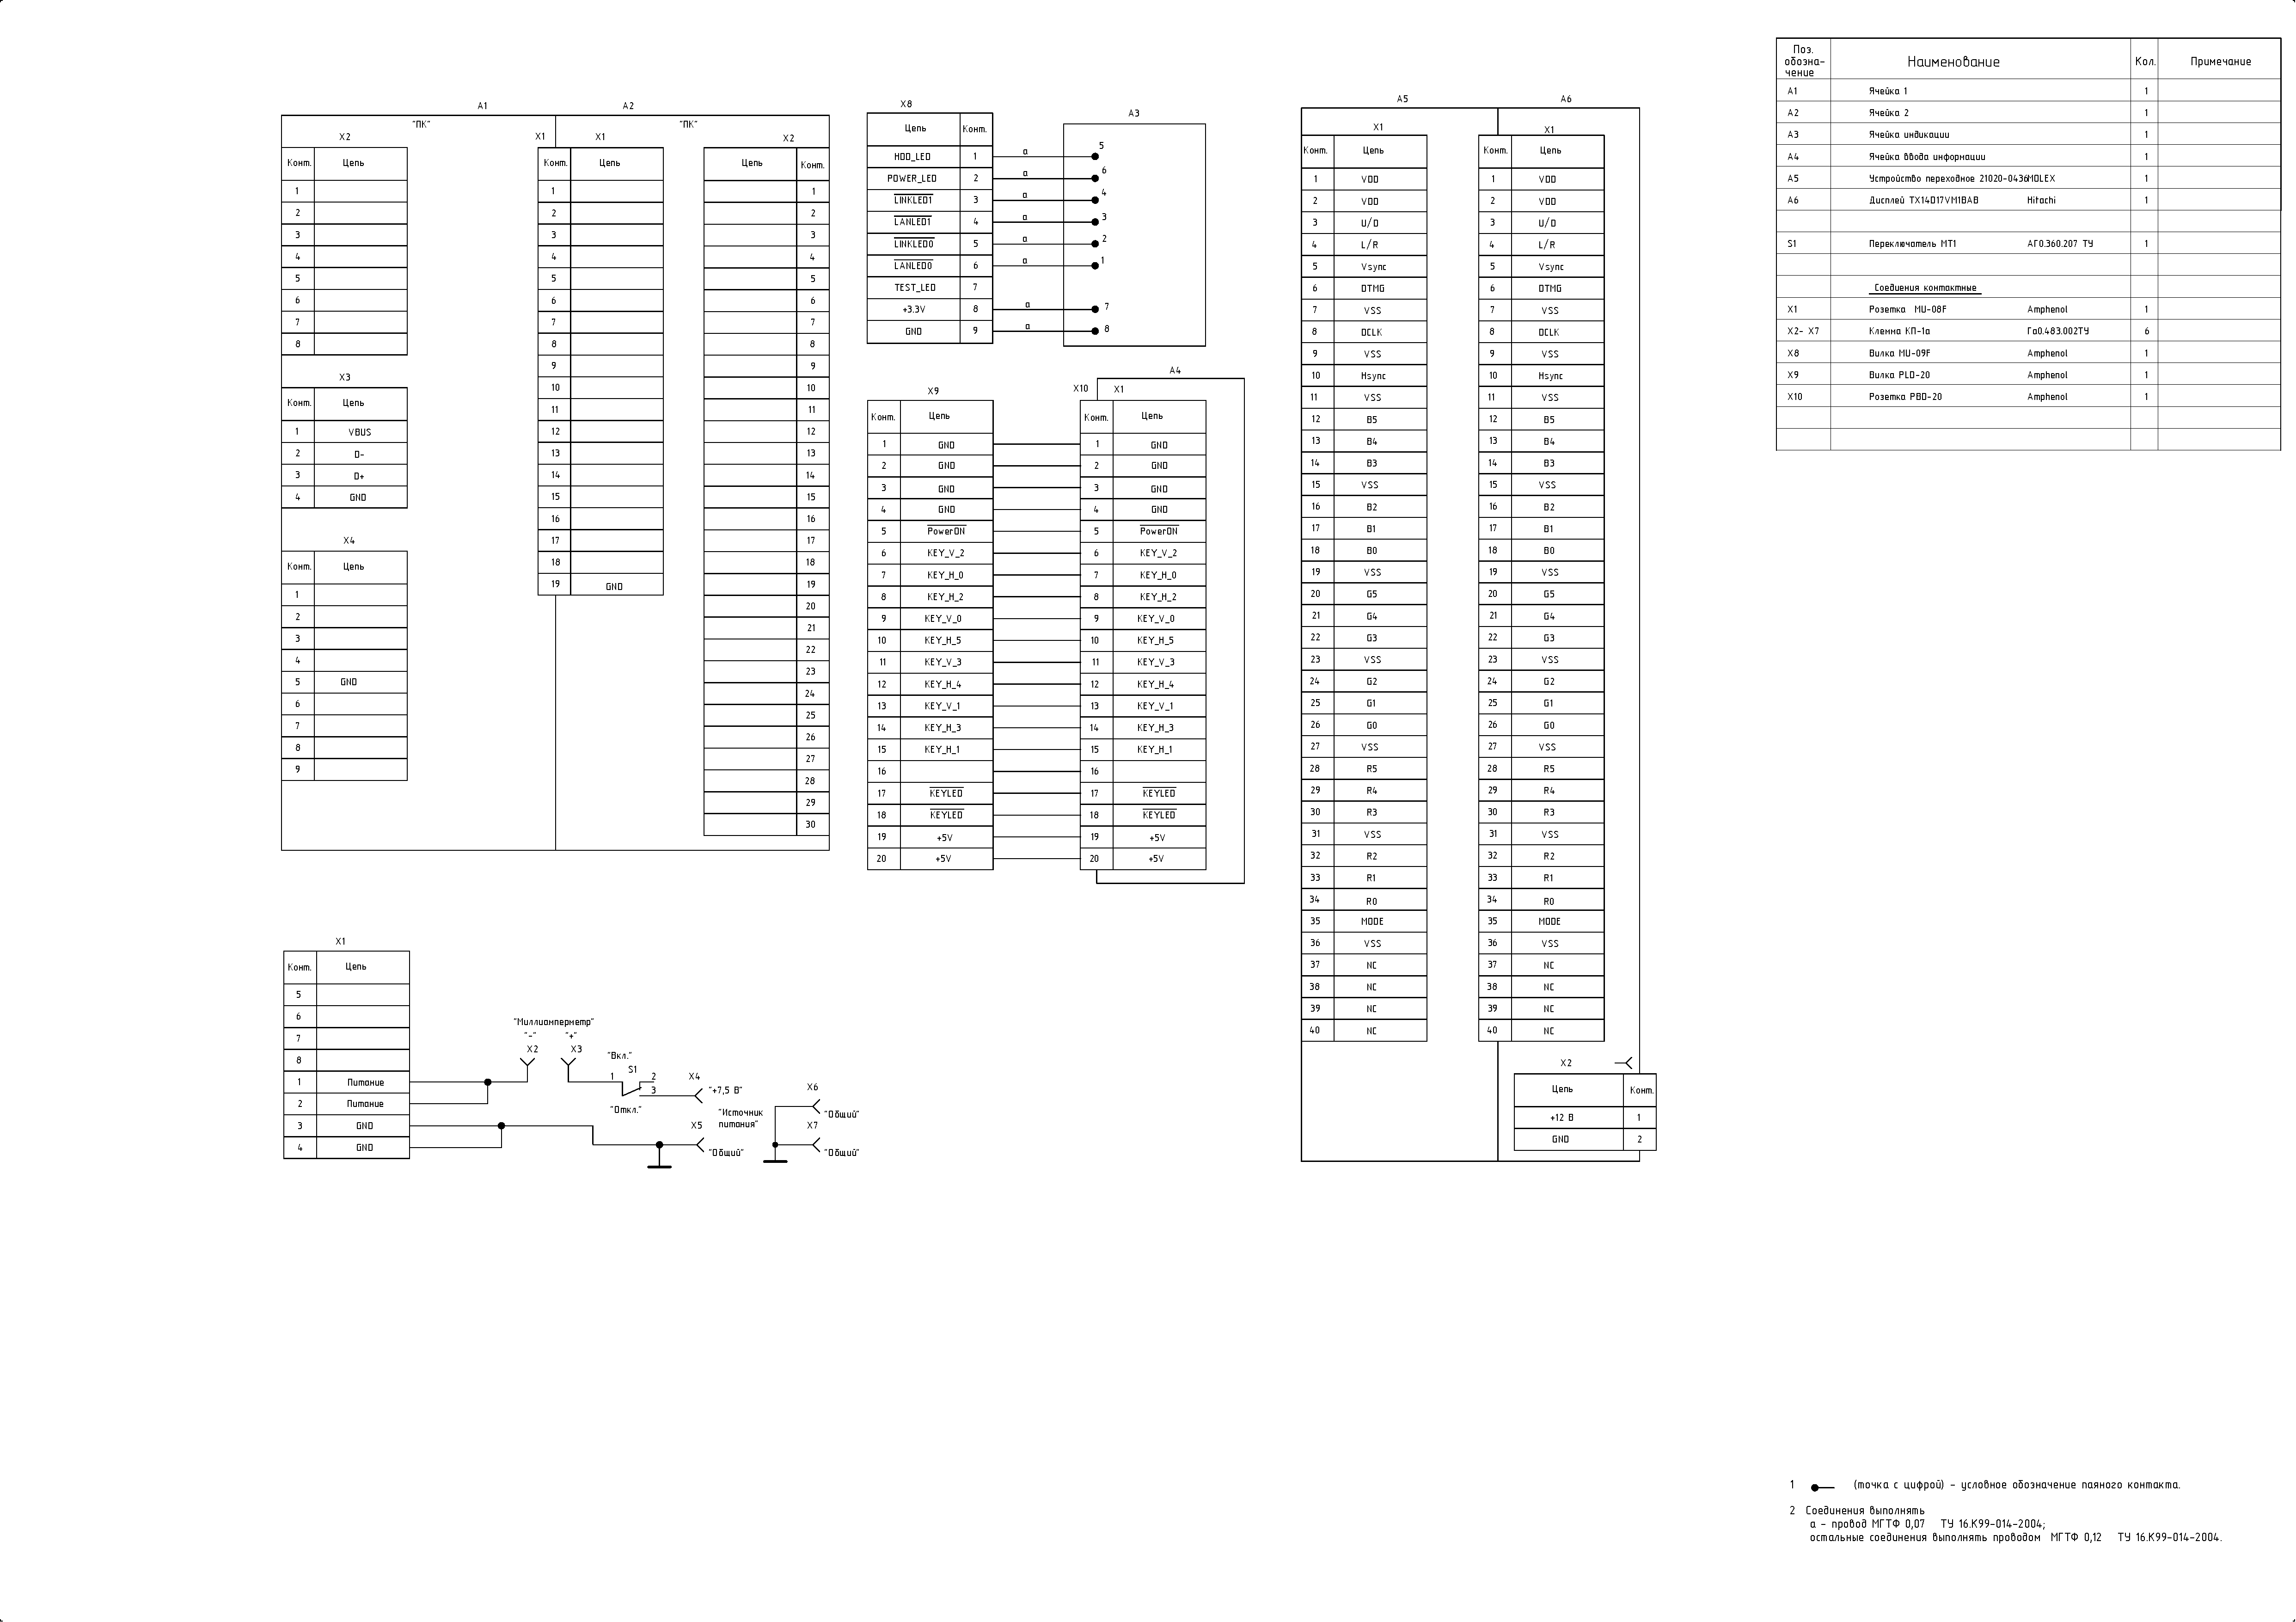
\includegraphics[scale=1,  angle=0]{./about/A1_example}}% Волшебные чиселки. Их лучше не трогать, а то картинки расползутся и подпись к рисунку уползёт
    \spboxmm{330}{40}{330}{40}{lc}{\parbox{100mm}{\caption{Схема электрическая принципиальная пульта для программирования} \label{a:p:pult_main}}}
  \end{picture}%
\end{figure}%
}%


\FormatSizeA{2}{%
\begin{figure}[H]%
  \unitlength=1mm%
  \begin{picture}(0, 330)(25,80)% Волшебные чиселки. Их лучше не трогать, а то картинки расползутся и подпись к рисунку уползёт
    \put(0,0){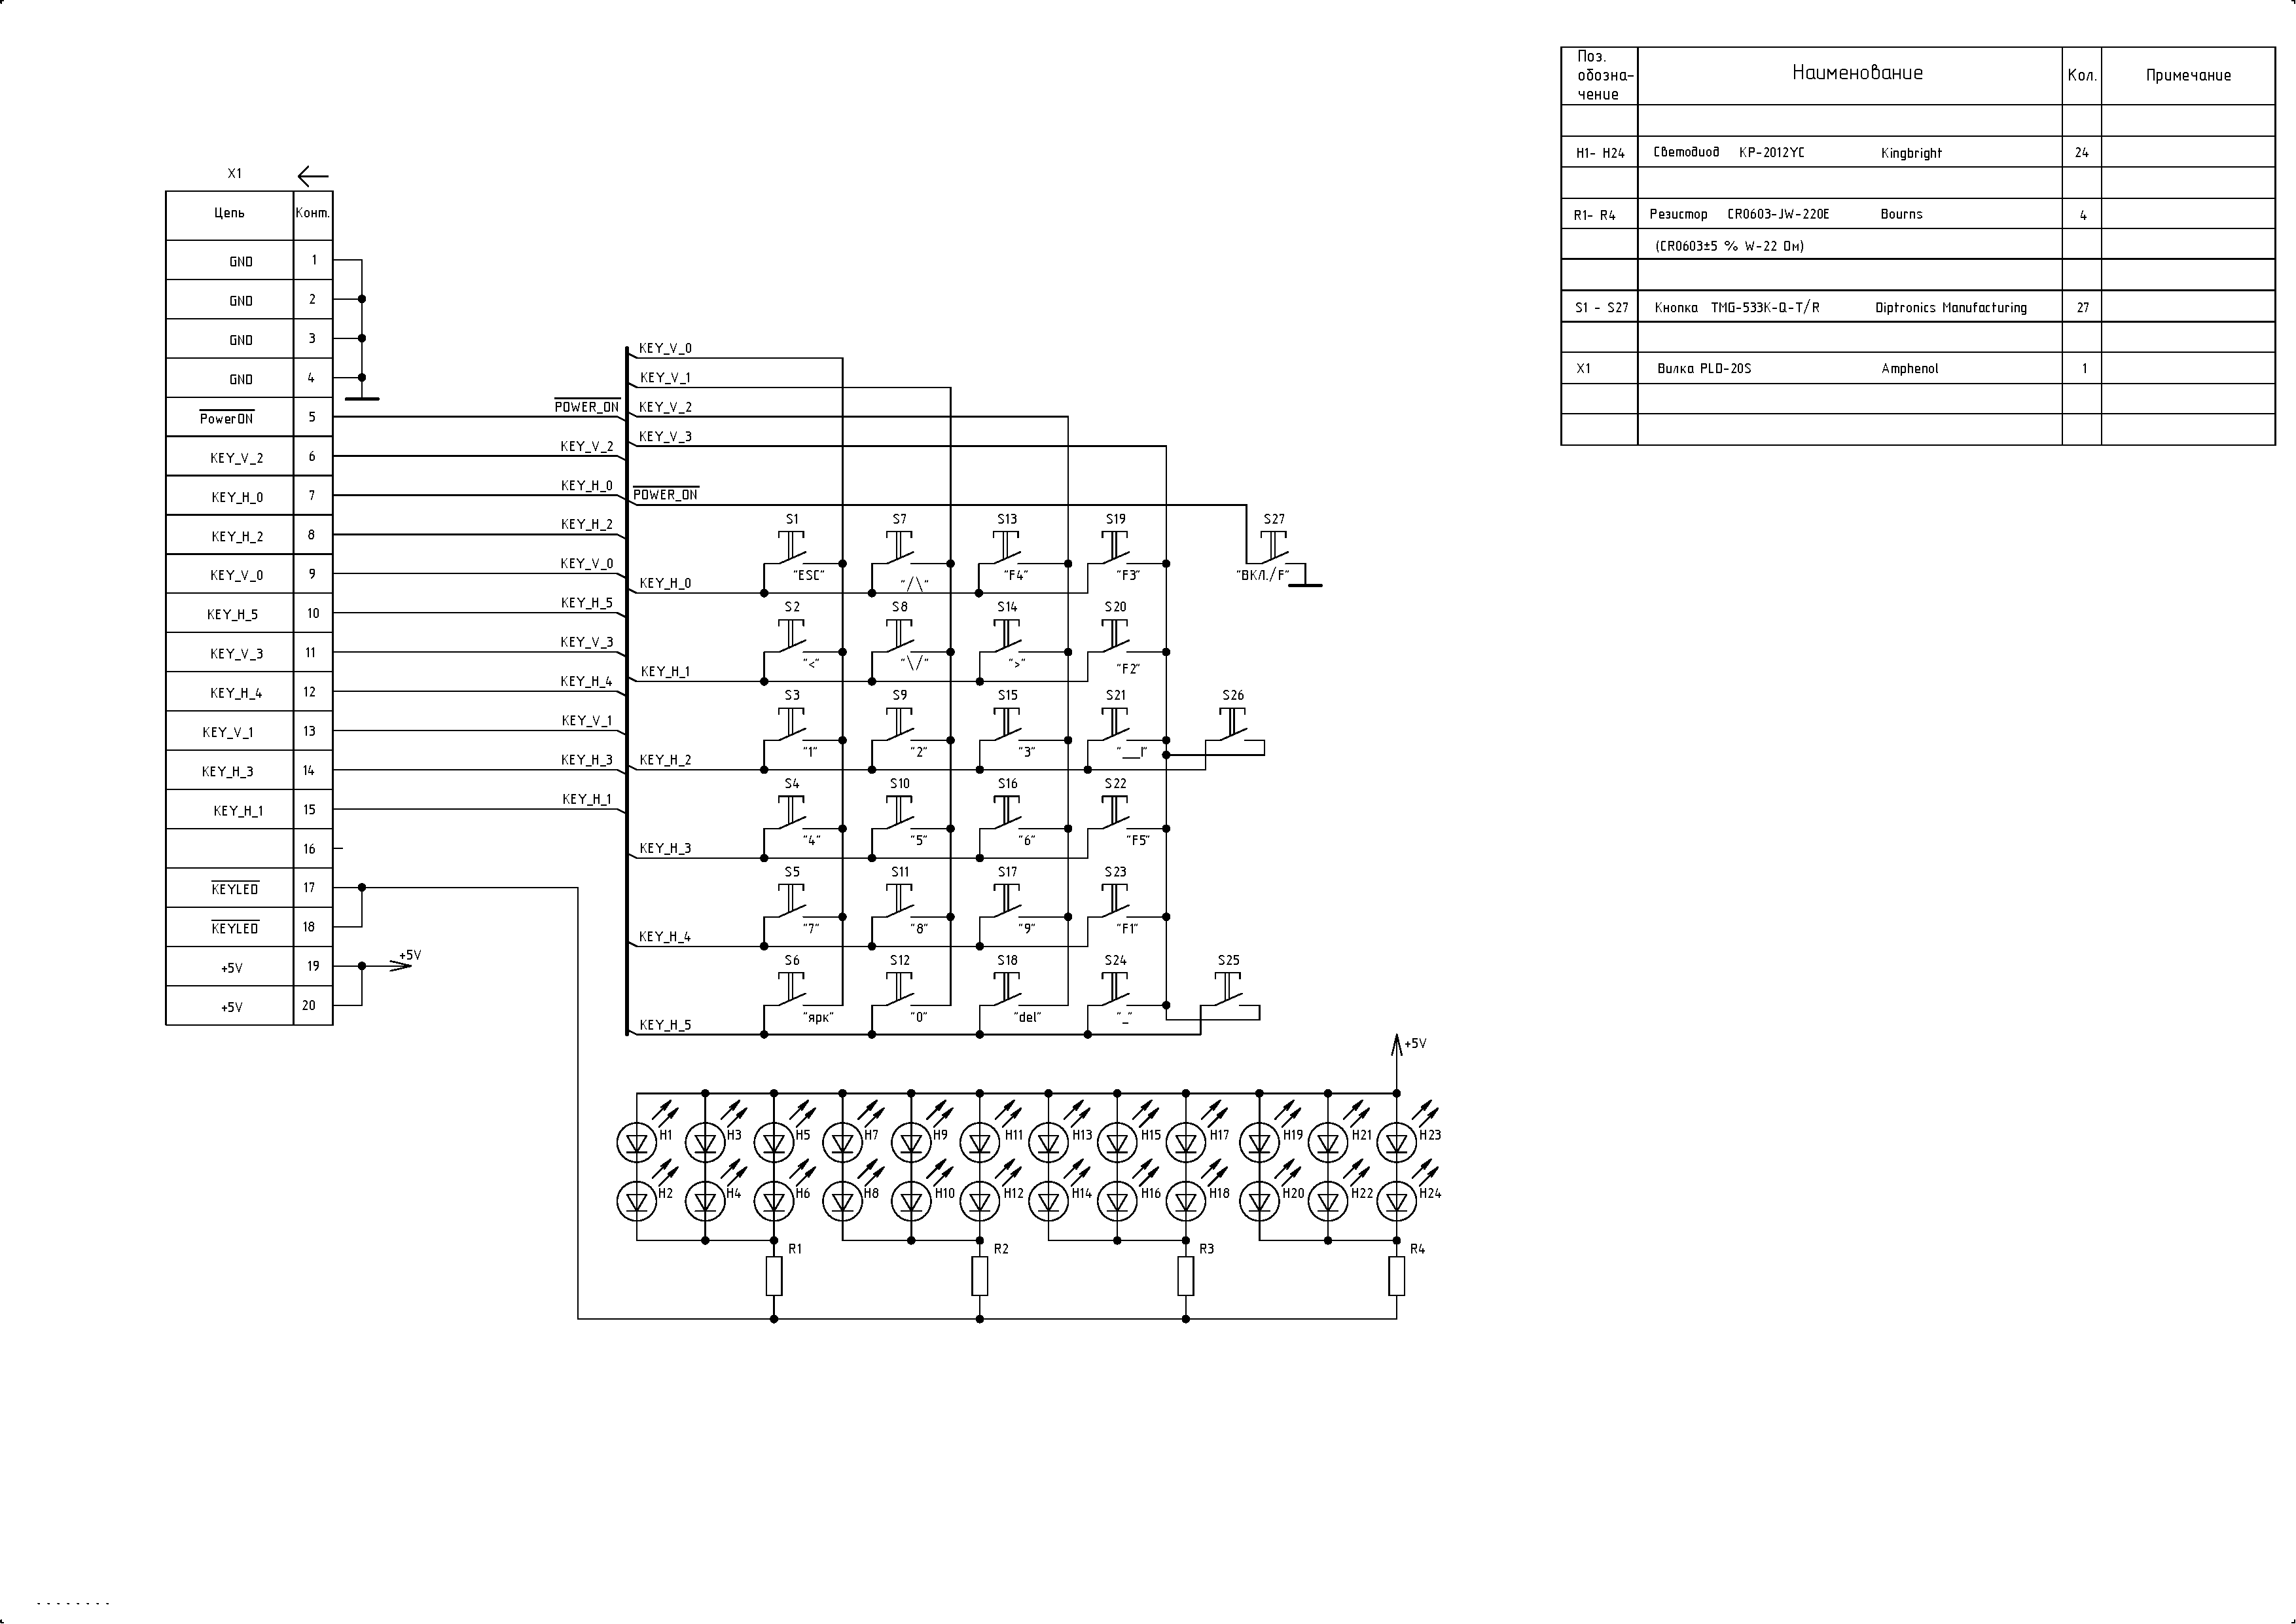
\includegraphics[ scale=1, angle=0]{./about/A2_example}}% Волшебные чиселки. Их лучше не трогать, а то картинки расползутся и подпись к рисунку уползёт
    \spboxmm{270}{30}{270}{30}{lc}{\parbox{100mm}{\caption{Схема электрическая принципиальная ячейки ввода информации}\label{a:p:pult_main_part1}}}
  \end{picture}%
\end{figure}%
}%


\begin{figure}[H]% 
\unitlength=1mm%
  \begin{picture}(0,235)(25,50)% Волшебные чиселки. Их лучше не трогать, а то картинки расползутся и подпись к рисунку уползёт
    \put(0,0){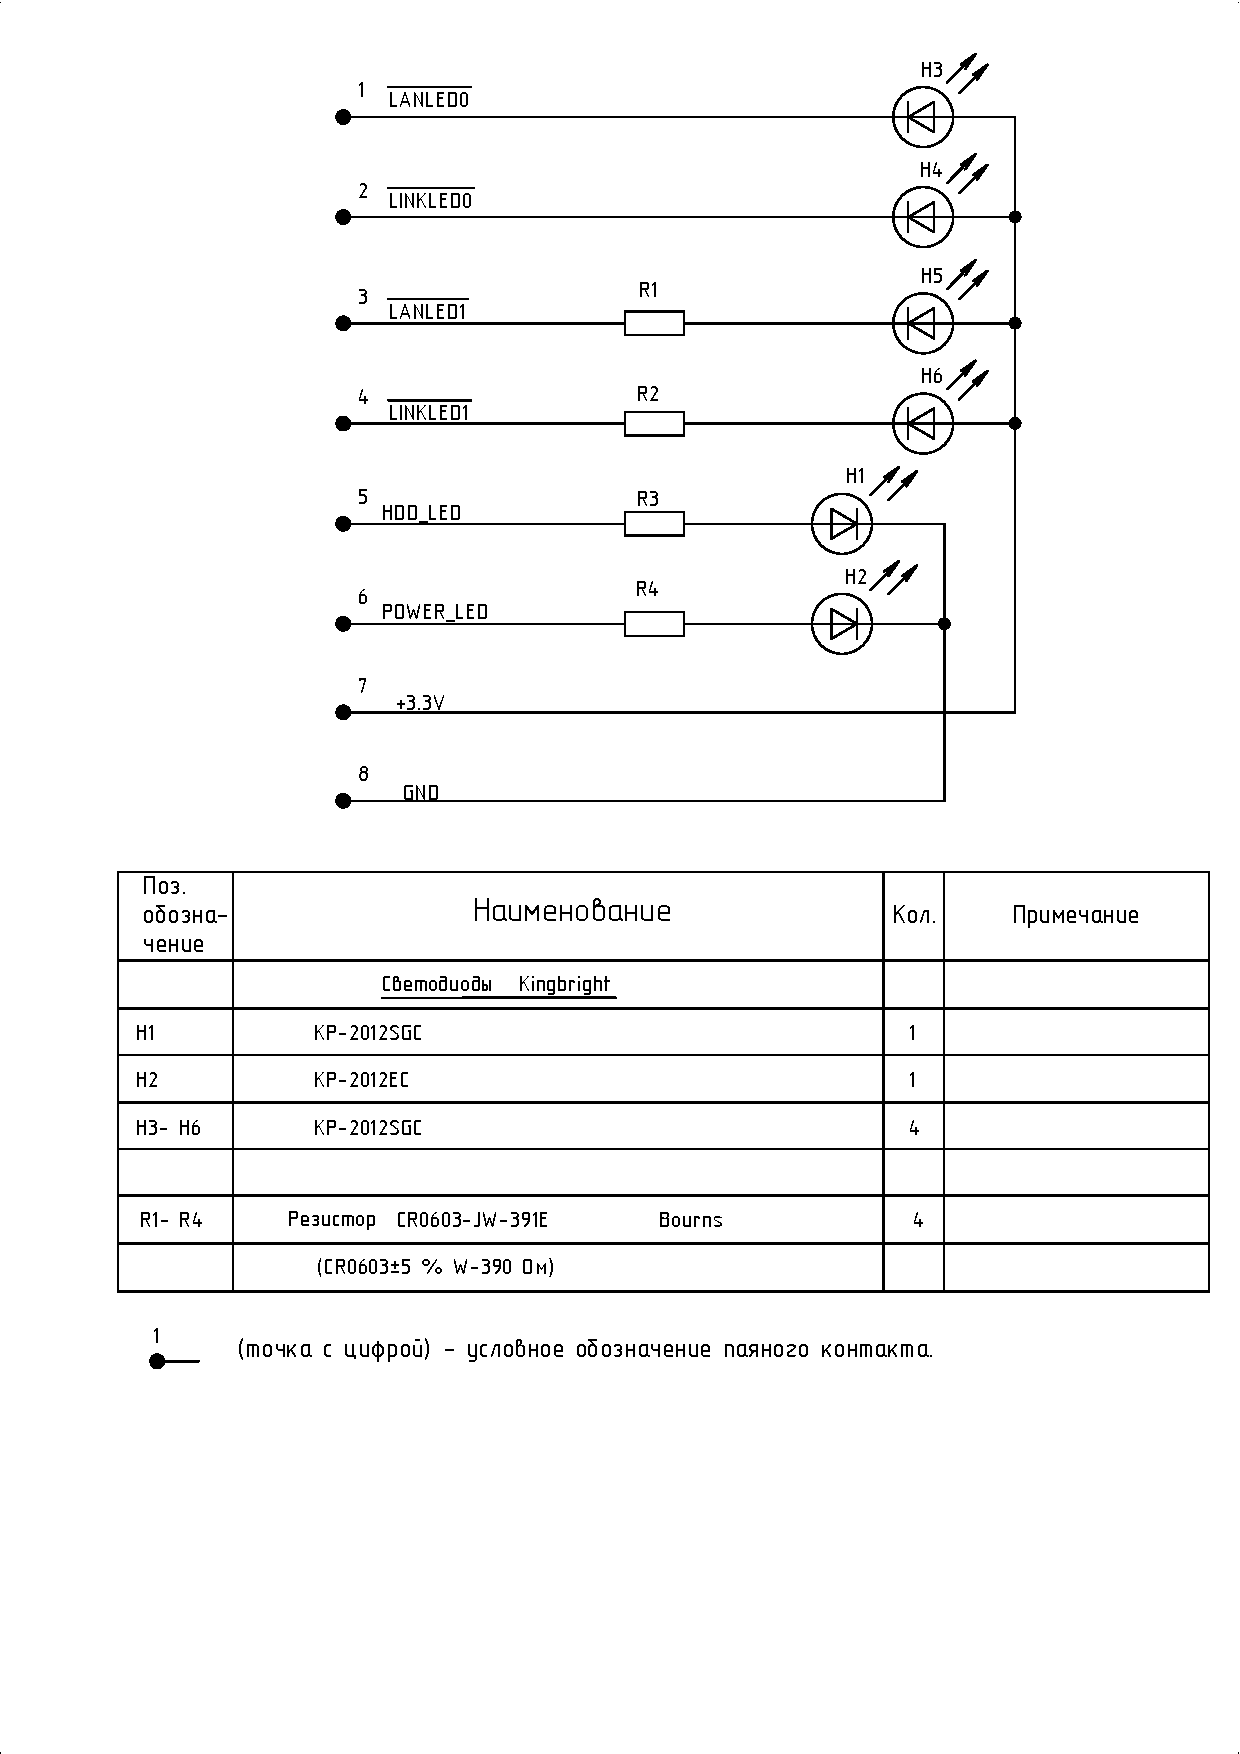
\includegraphics[scale = 1.004]{./about/A4_v_example}}% Волшебные чиселки. Их лучше не трогать, а то картинки расползутся и подпись к рисунку уползёт
    \spboxmm{60}{40}{60}{40}{lc}{\parbox{100mm}{\caption{Схема электрическая принципиальная ячейки индикации} \label{a:p:pult_main_part2}}}
  \end{picture}%
\end{figure}%


\FormatSizeA{3}{% 
%\section {Схема электрическая подключения устройства} \label{app:SCH_all_units}
\begin{figure}[H]%
\unitlength=1mm%
  \begin{picture}(0,230)(25,45)% Волшебные чиселки. Их лучше не трогать, а то картинки расползутся и подпись к рисунку уползёт
    \put(0,0){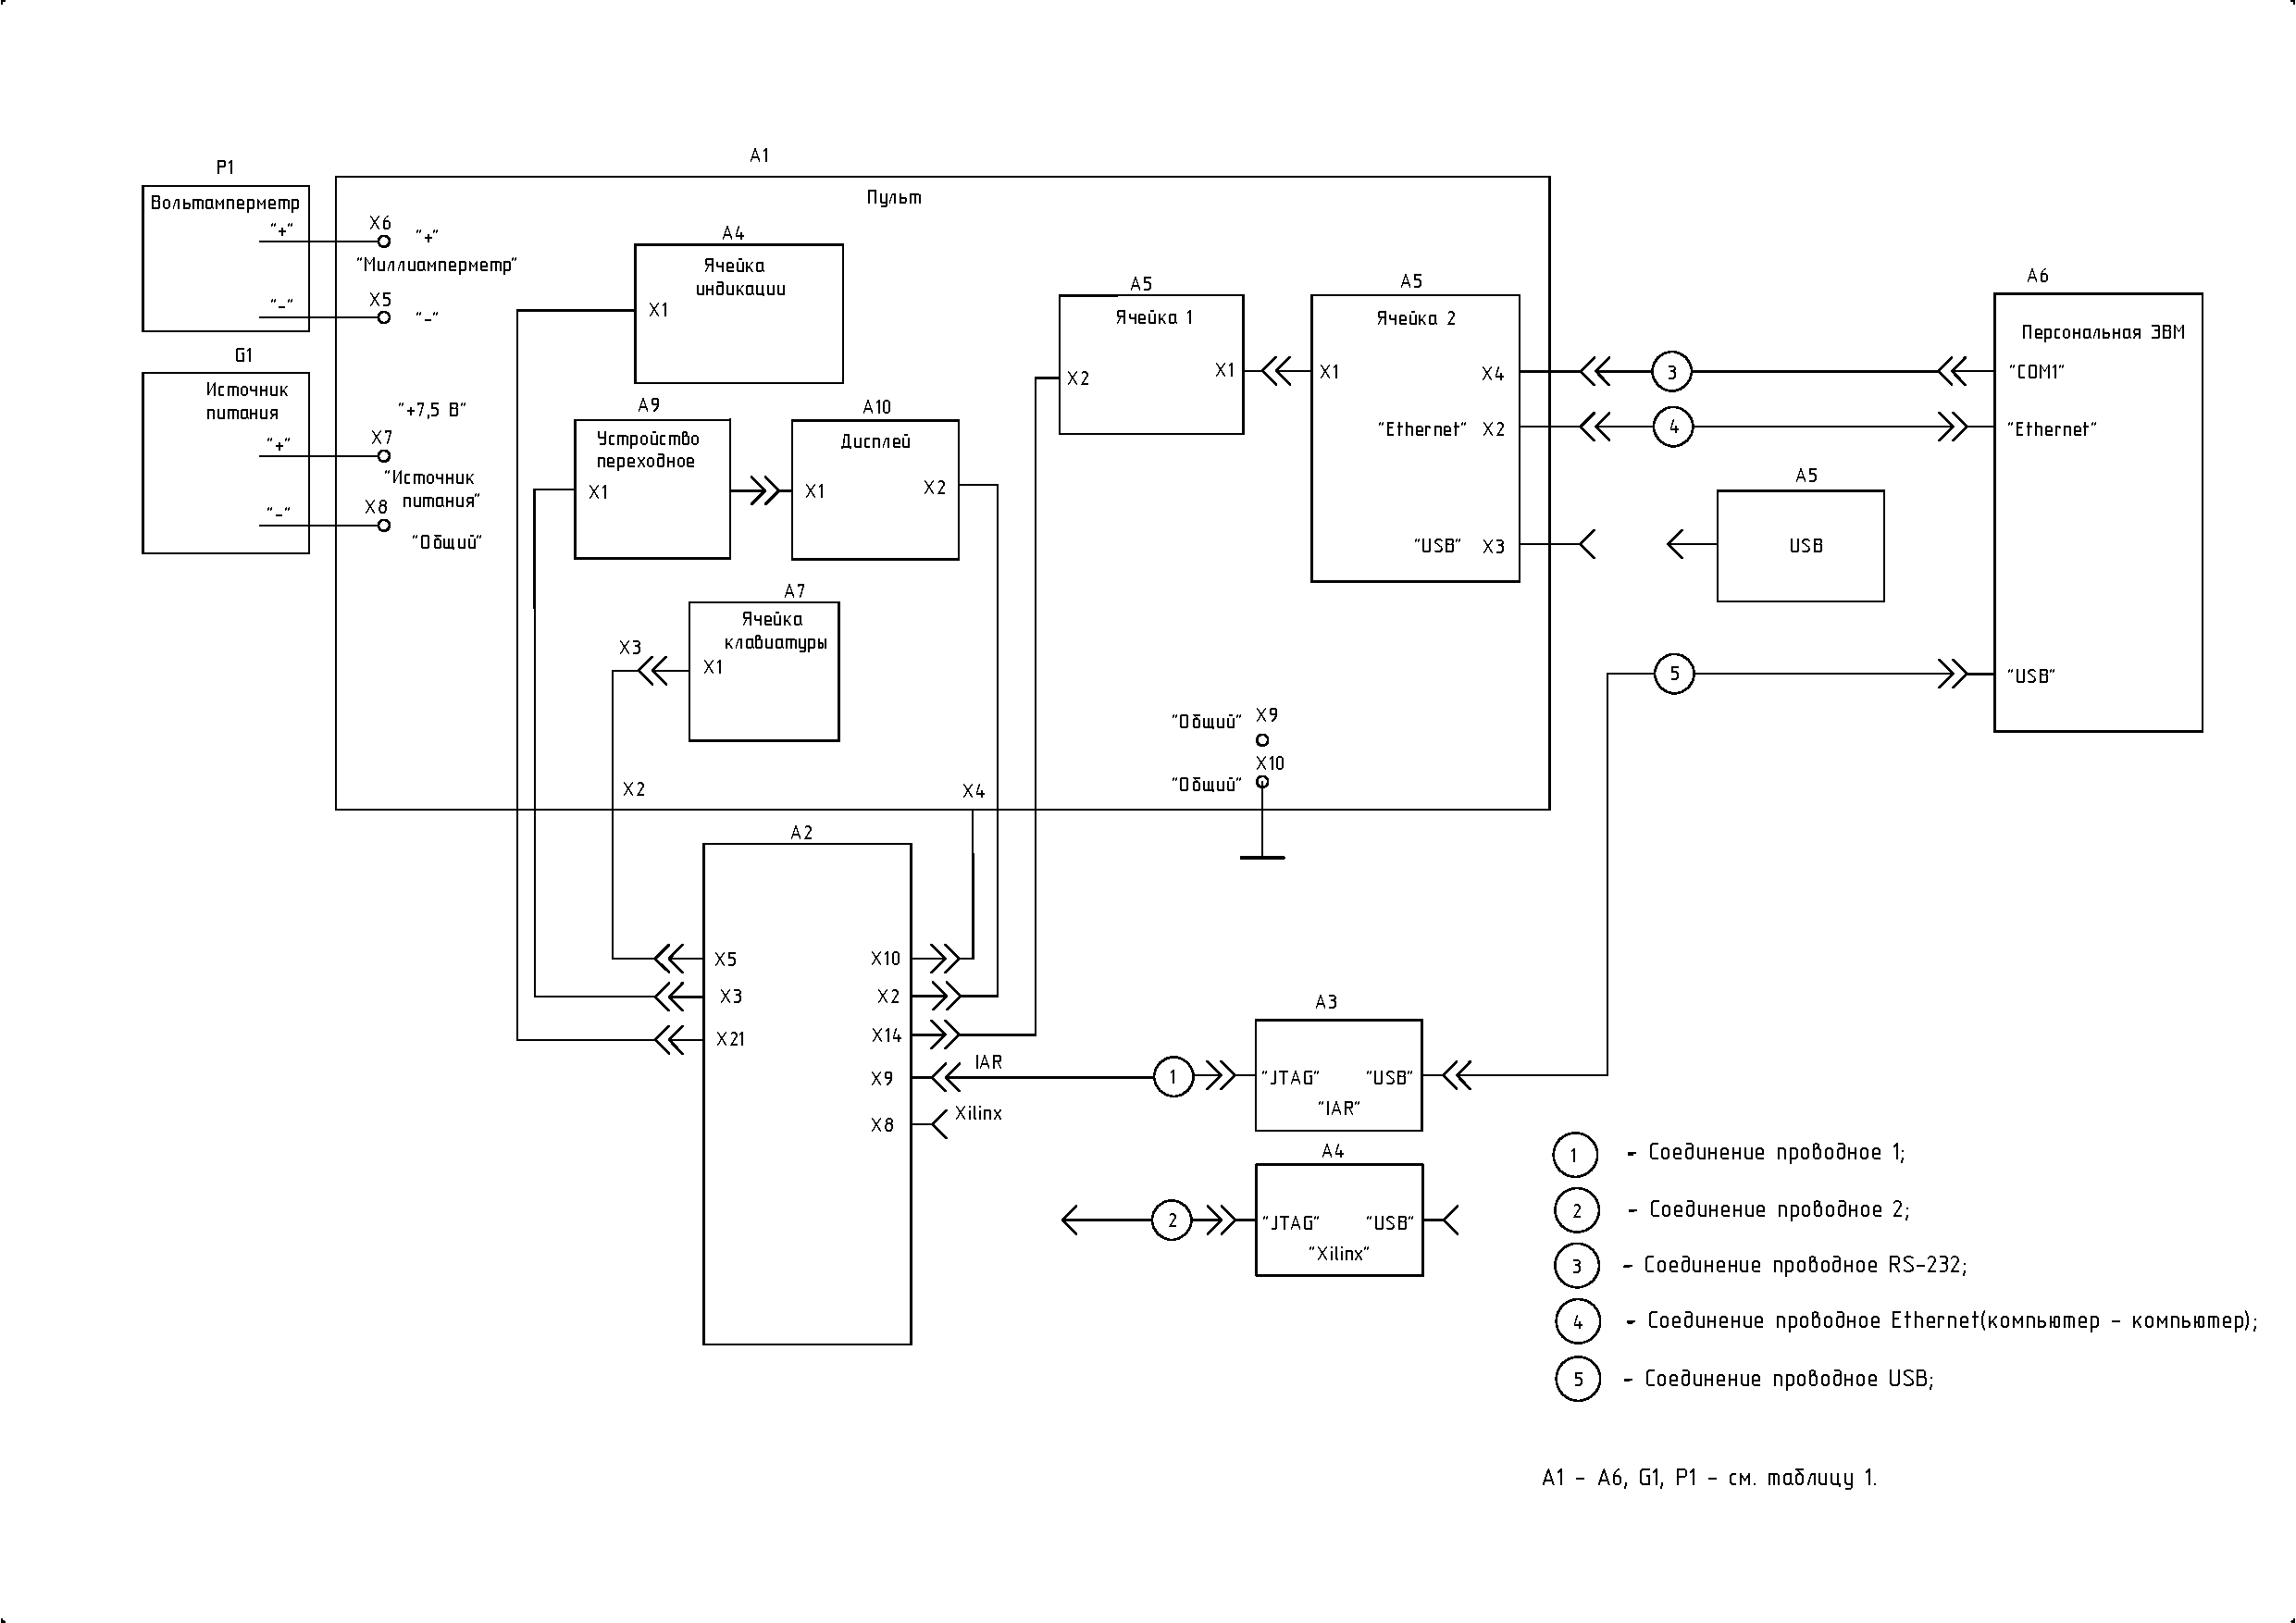
\includegraphics[ scale=1, angle=0]{./about/A3_example}}% Волшебные чиселки. Их лучше не трогать, а то картинки расползутся и подпись к рисунку уползёт
    \spboxmm{160}{20}{160}{20}{lc}{\parbox{100mm}{\caption{Схема электрическая подключения устройства} \label{a:p:SCH_all_units}}}
  \end{picture}%
\end{figure}%
}%










\FormatSizeA{3}{%
\section {Схема электрическая подключения устройства} \label{app:SCH_all_units}
\begin{figure}[H]%
\unitlength=1mm%
  \begin{picture}(0,200)(25,56)% Волшебные чиселки. Их лучше не трогать, а то картинки расползутся и подпись к рисунку уползёт
    \put(0,0){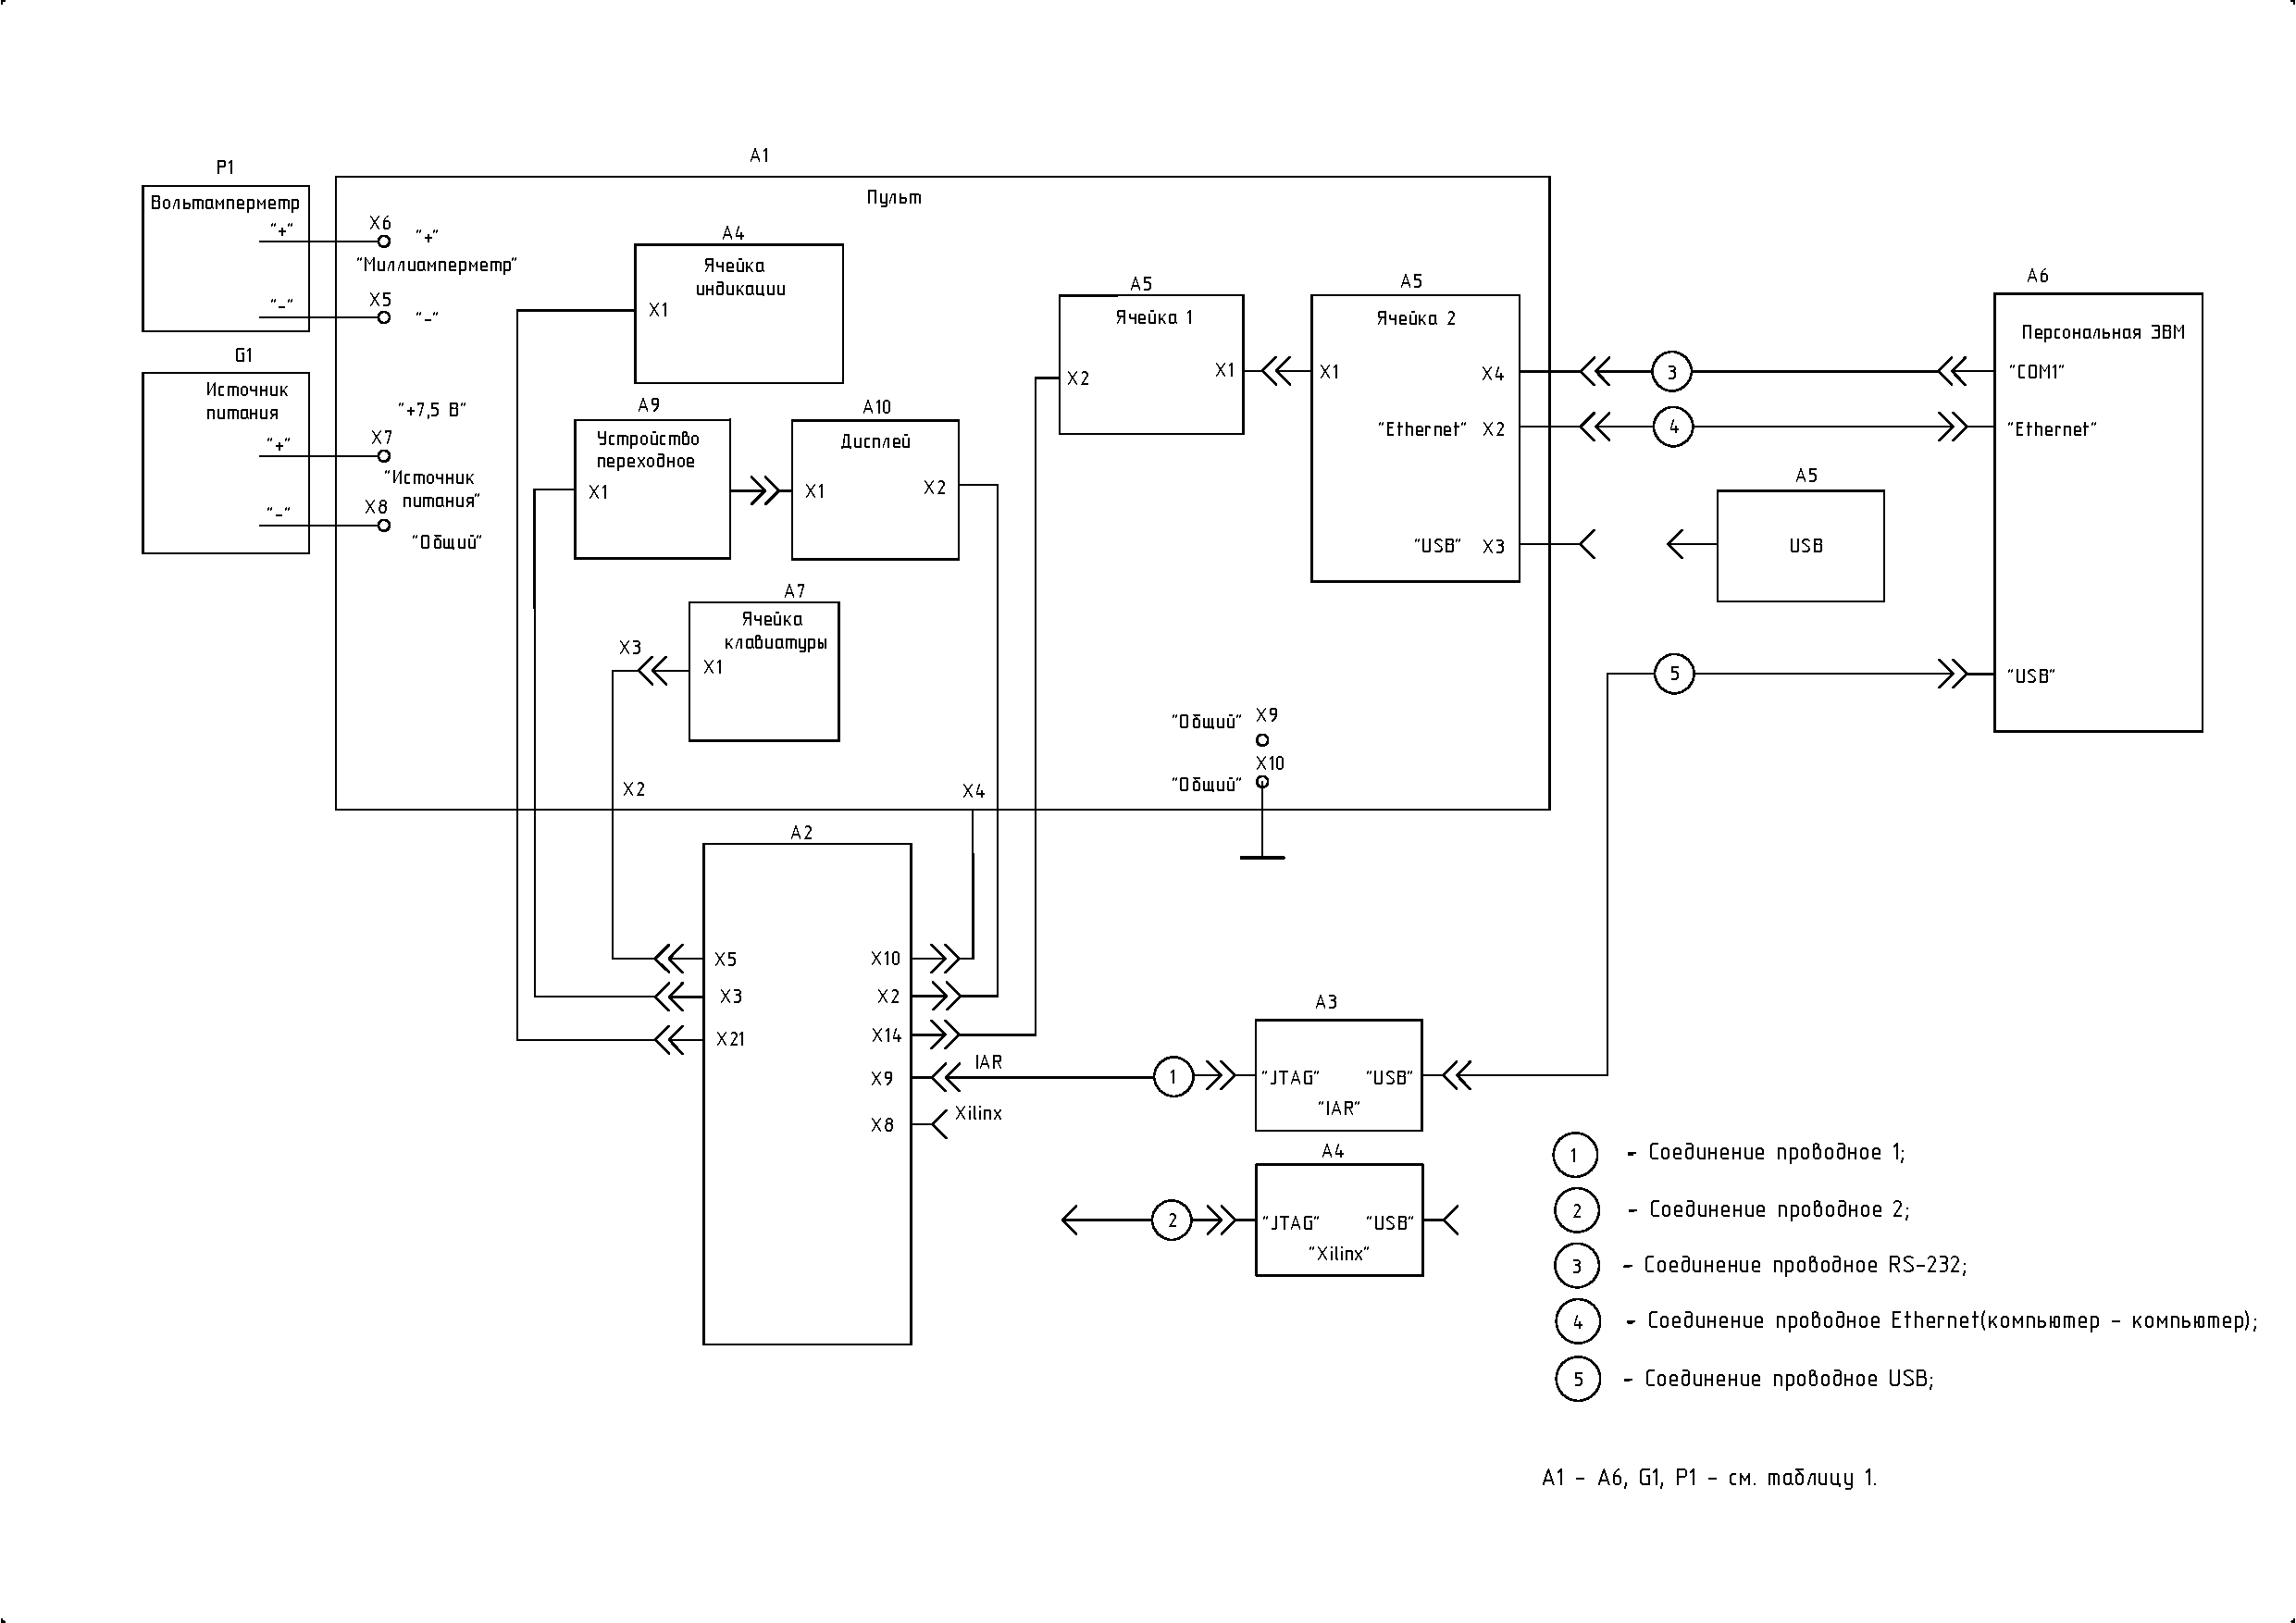
\includegraphics[ scale=1, angle=0]{./about/A3_example}}% Волшебные чиселки. Их лучше не трогать, а то картинки расползутся и подпись к рисунку уползёт
    \spboxmm{160}{30}{160}{30}{lc}{\parbox{100mm}{\caption{Схема электрическая подключения устройства} \label{a:p:SCH_all_units}}}
  \end{picture}%
\end{figure}%
}%




\FormatSizeA{43}{%
\begin{figure}[H]%
\unitlength=1mm%
  \begin{picture}(0,235)(-60,50)% Волшебные чиселки. Их лучше не трогать, а то картинки расползутся и подпись к рисунку уползёт
    \put(0,0){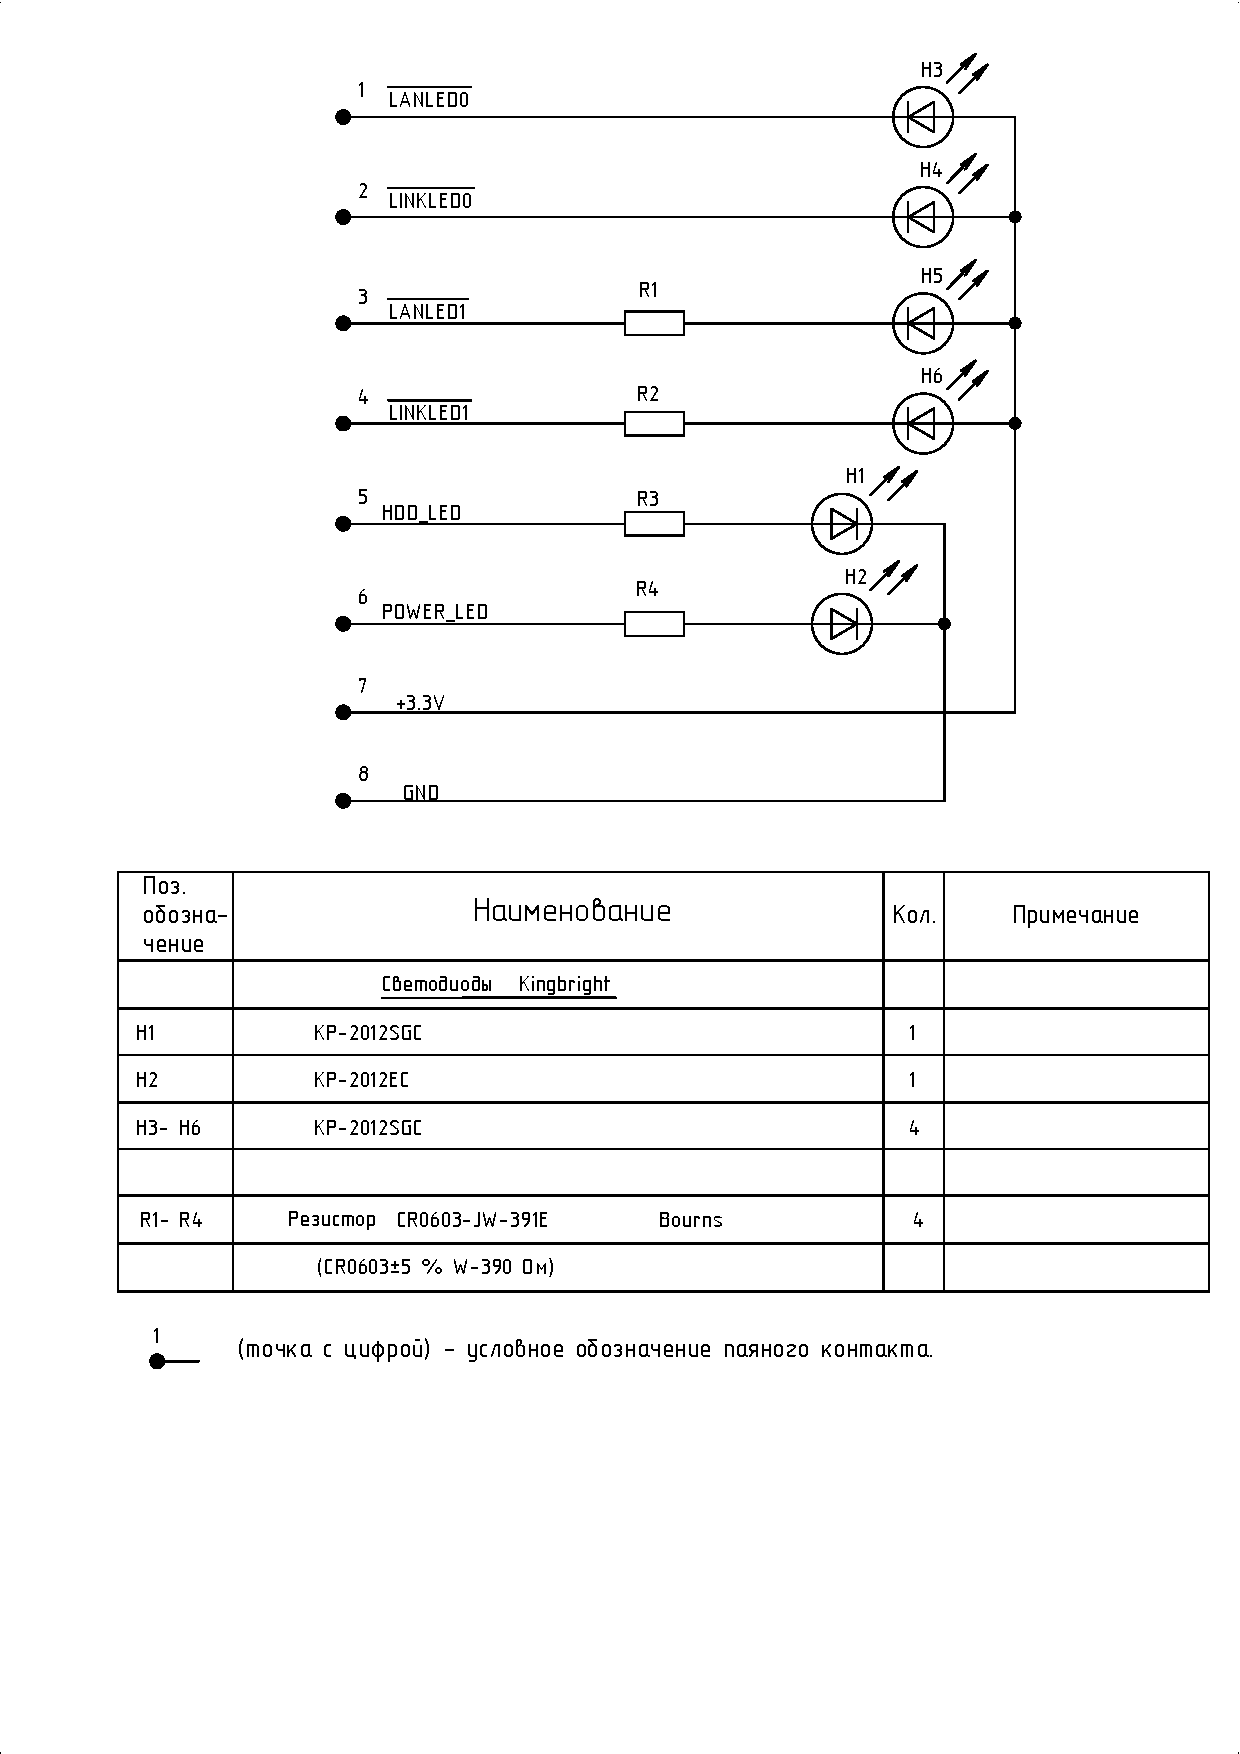
\includegraphics[scale = 1.004]{./about/A4_v_example}}% Волшебные чиселки. Их лучше не трогать, а то картинки расползутся и подпись к рисунку уползёт
    \spboxmm{160}{30}{160}{30}{lc}{\parbox{100mm}{\caption{Схема электрическая принципиальная ячейки индикации} \label{a:p:pult_main_part20}}}
  \end{picture}%
\end{figure}%
}%







